\documentclass[12pt,a4paper]{article}

% Packages
\usepackage[utf8]{inputenc}
\usepackage{graphicx}
\usepackage{amsmath}
\usepackage{amsfonts}
\usepackage[hidelinks]{hyperref}
\usepackage{geometry}
\geometry{margin=1in}
\usepackage{ulem}

% Title and Author
\title{Robotics Project}
\author{Benassi Alessandro, Calvo Daniele, Cristoforetti Niccolò, Gottardelli Matteo}
\date{\today}

% Begin Document
\begin{document}

% Title Page
\maketitle
\tableofcontents
\newpage

%Introduction
\section{Introduction}\label{sec:intro}
This paper describes the methodology and the results achieved by a ros2 based program that moves an UR5 robotic arm with a gripper, in order to grab and move some different randomly spawned blocks from a random start position to a desired position. The aim of this project is to provide a functional and correct implementation to be able to perform the operation without encountering singularities or errors.\\
Different instrumentation was used to develop the project, starting from the blocks to move, and the camera, which allows us to scan an image on which we can perform detection and determine the position and the orientation of the objects. The last fundamental component is the UR5 robotic arm, a lightweight arm designed for tasks that require flexibility; it has 6 degrees of freedom and is composed by revolute joints: a base, a shoulder, an elbow and a spherical wrist.\\
Regarding the development environment, different tools were used. The first is DockerDesktop which allows us to run the image provided by the professor. It is an Ubuntu virtual machine with ros2 on it. This allows us to use nodes and services for communication between the different parts. The Eigen and yolov5-pip libraries are used and the necessary Python modules are downloaded when starting the program. There is also the Roboflow application which is used to generate pre-trained weights for the recognition part.\\ 
The algorithm developed is divided into two main parts: vision and manipulation. The first is responsible of scanning the camera to extract an image, process it to localize all the blocks using Yolov5 and returning the coordinates of the bounding boxes to calculate the relative positions. The second controls the movement of the arm to reach the given position, grab the object and put it in the designed position.


% Vision Section
\section{Vision}\label{sec:vision}
Vision plays a critical role in robotics by allowing the robot to perceive and interpret its environment. 
The three main challenges for this project are: spawning the blocks, recognizing them, and calculating their position in the space.

\subsection{Block spawn}\label{subsec:blockspawn}
As mentioned in \ref{sec:intro} the absolute position is the one of the camera, given by the following parameters: x=-0.5 , y=0.5, z=1.2, R=0.0, P=0.4, Y=-0.06, the first three are the coordinates, the others are the rotation values. At this point we had the table with the arm attached, and we wanted to spawn the blocks in the right part, which is closer to the camera. The blocks are spawned directly in the sim.launch.py so they are spawned right after the creation of the environment with the table and the arm\uline{(non del tutto vero guardando LaunchDescription)}. The minimum number of blocks \uline{is 1 and it goes up to 9} and this parameter is inserted by the user in the command line. The spawn area of the blocks has a fixed height, which is based on the one of the table (z=0.88) and \uline{its width in the x and y axis is respectively (0.05, 0.405) and (0.2, 0.58)}. All the generated blocks are different in type and color. The type is decided randomly between a set of nine, taken from the ones in the folder published on moodle, which were eleven, but we decided to remove two of them that are larger than the single block to avoid issues with the gripper, that may not open enough to get around the block, \uline{since the script we are in posses only allows us to open and close and not to decide a width}. The color is also chosen in a random way between a selected set and, regarding the position, it is generated randomly and has to stay within the limits of the defined spawn area and be collision free, so there is a minimum distance between each object, otherwise we regenerate the overlapping one. The orientation is random and is only about the roll(z axis), because the project does not consider the blocks in a different position, like upside down, for a matter of complications in detection and grabbing.
The objects are generated using a .urdf.xacro file, which is then passed to .urdf format and at the end in .sdf to be displayable on Gazebo. 


\subsection{Processing images}\label{subsec:imageproc}
To perform object recognition, the first thing to do is scan an image from the camera. This is done by the node image\_acquiring, which subscribes to the topic that publishes \textit{sensor\_msgs::msg::Image} data and, after gathering the content, it is processed with opencv2 library functions to print it on a generated image file in .png format. It is saved in a precise path, that will be used later in the program.\\Since recognition is performed at every complete movement of the arm, the part of the table with the blocks that have already been moved is darkened to avoid the recognition and movement of these. Furthermore, the background is colored black to allow the object recognition algorithm to perform at its best.
\begin{center}
    \begin{figure}
        \centering
        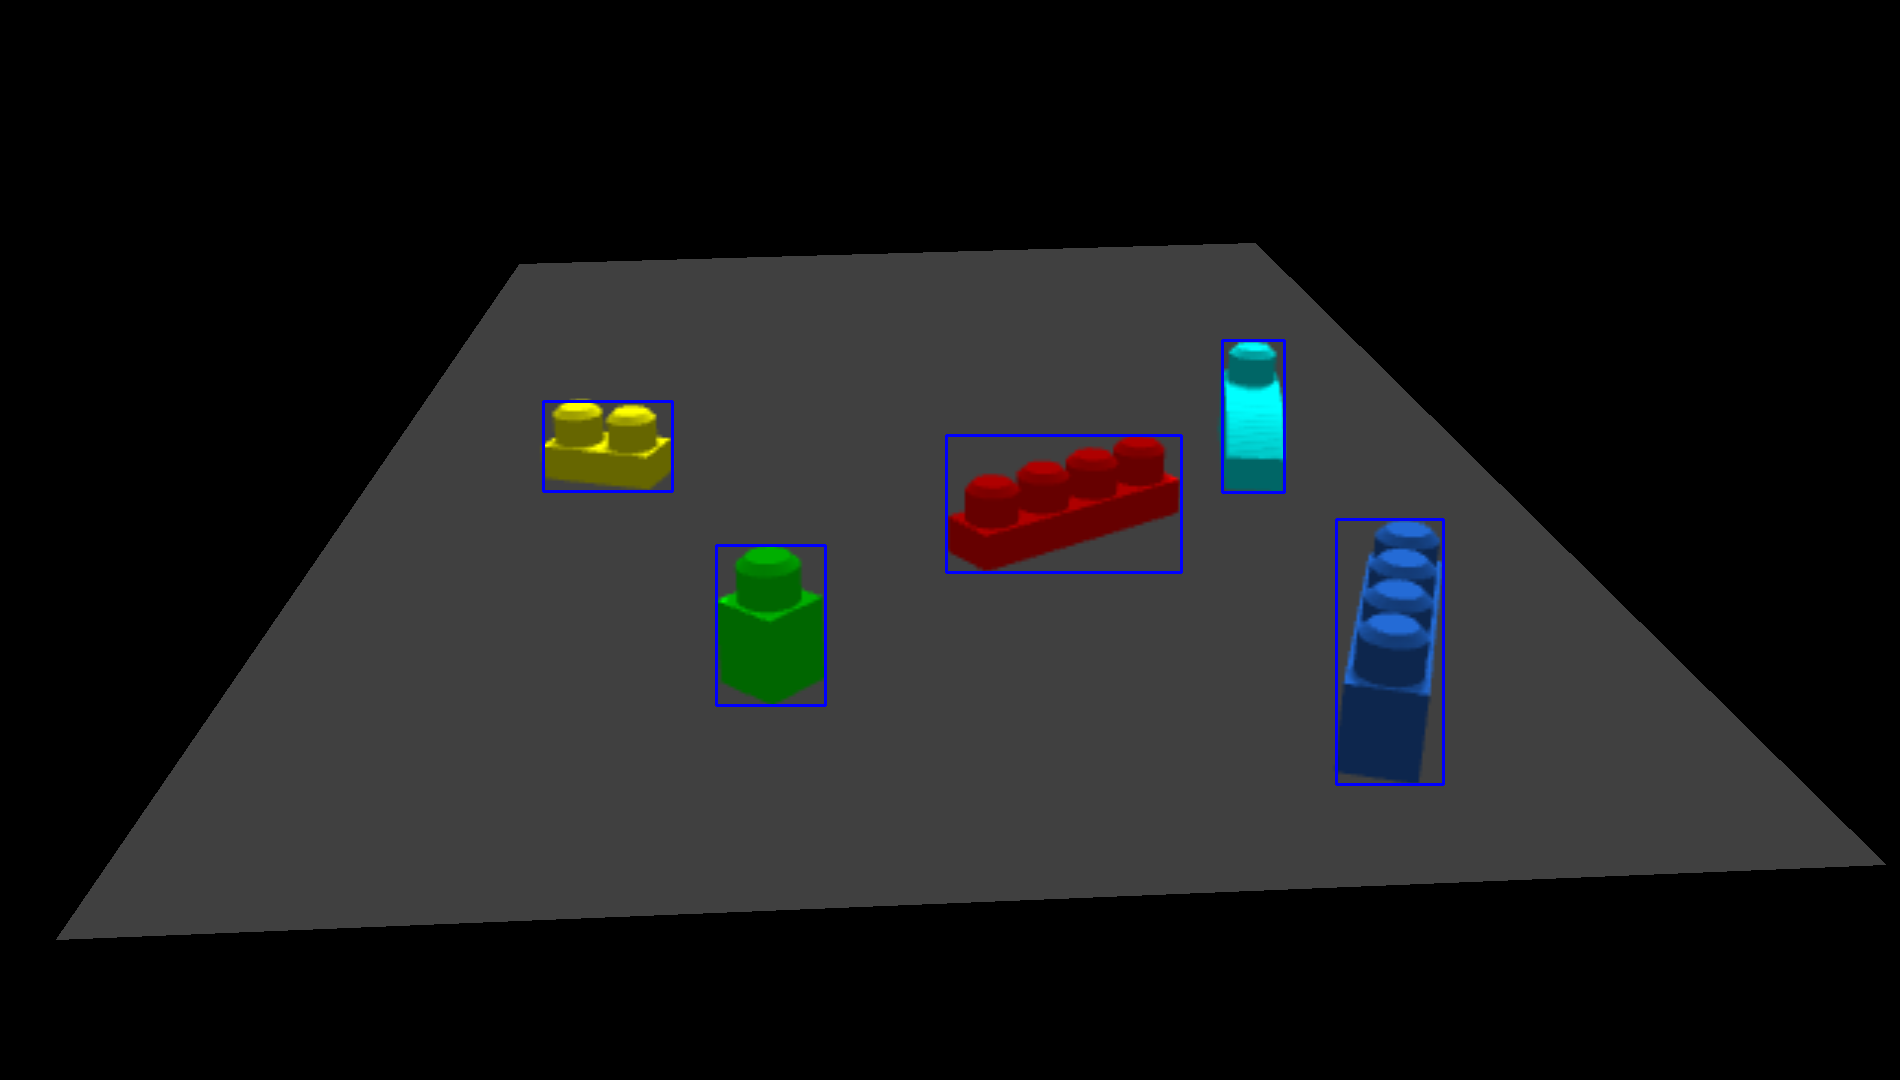
\includegraphics[width=1.0\columnwidth]{images/Yolo1.png}
        \caption{Blocks detection with bounding-boxes}
        \label{fig:yolo1}
    \end{figure}
\end{center}

\subsection{Detection}\label{subsec:detect}
For this part we used the Roboflow tool which allowed us to process the images and detect objects in order to produce a pre-trained weight file \uline{for Yolov5}. \uline{The images used were the ones provided by the professor, excluding the .json files that were unuseful since we decided to create our own dataset from scratch.} To do that, we uploaded the files on the tool and analyzed them folder by folder, telling the program which class it is. We ended up having nine classes(see \ref{subsec:blockspawn}), each with a \uline{large} number of images loaded. Then a percentage of images was destined to training, and a smaller one to testing, this was done automatically by the program, which performed also the training part. At the end of the processes the program output was \uline{blocktrain.pt}, which is the file containing the pre-trained weights to be used to perform the recognition with Yolov5. 
For the recognition the yolov5-pip repository is downloaded from github (link: \url{https://github.com/fcakyon/yolov5-pip.git}).\\
When passing an image we were interested in knowing the coordinates of the bounding box, the confidence, and the class. With the first one we are able to calculate the position of the block on the table and with the second one we can understand whether it is an erroneous identification. To obtain this information, we developed a Python script detection.py that creates the service: yolo\_bounding\_box\_service, which takes in input the path of the image from the camera, taken as explained in \ref{subsec:imageproc}, and returns an array of custom msg type called Boundstruct, that contains the class identifier, the confidence and the four values of the coordinates of the top left and bottom right points of the bounding box.
\begin{center}
    \begin{figure}
        \centering
        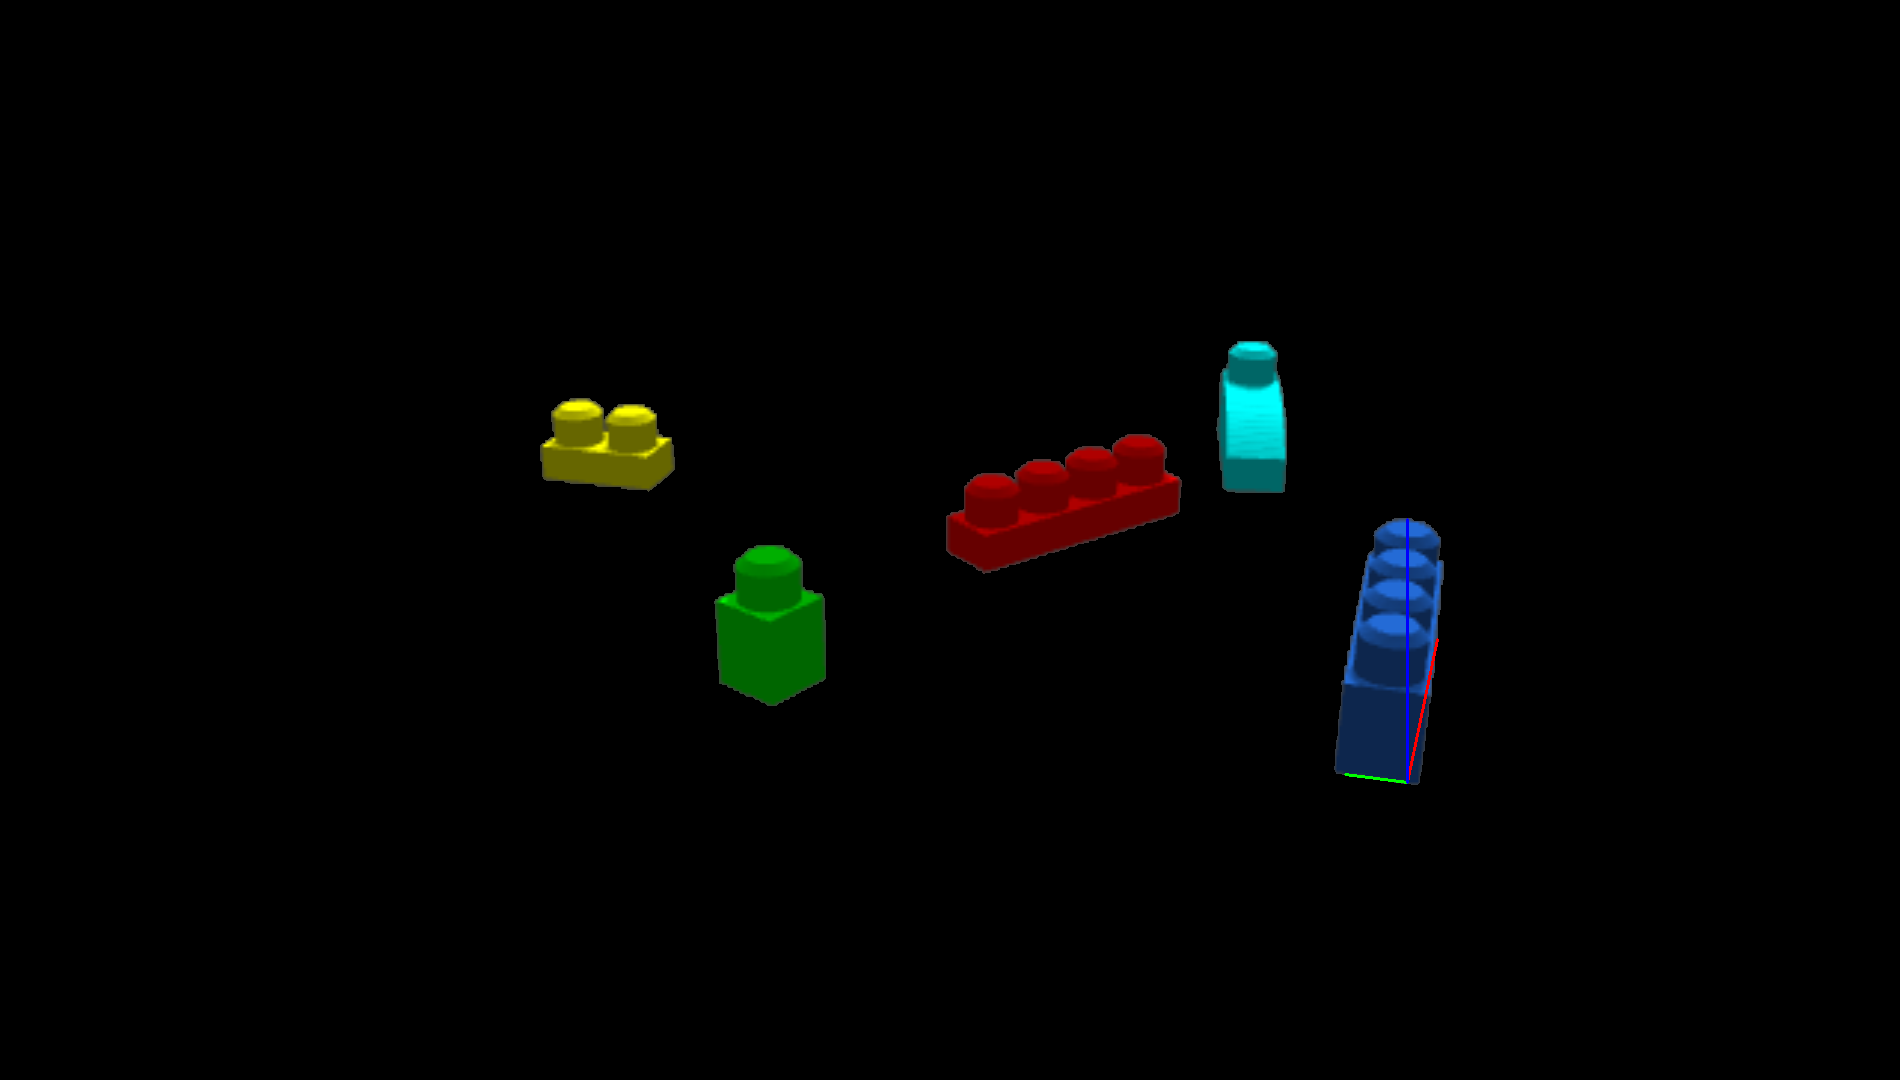
\includegraphics[width=1.0\columnwidth]{images/Obj1.png}
        \caption{Axis for the block to determine the orientation}
        \label{fig:obj1}
    \end{figure}
\end{center}
% Object elaboration Section
\subsection{Object elaboration}\label{subsec:objel}
\uline{da sistemare, credo che il Converison non serva più}
The values returned in \ref{subsec:detect}, in particular the coordinates of the bounding box, are essential to derive the center of the object and compute its distance from the camera. This is done using a function that determines the center by subtracting the further point coordinate with the lower ones, divide the difference by two and add it to the lower one values. Then the coordinates of this point are passed to the Conversion service which returns the depth. With this process we obtain the coordinates of the block with respect to the camera ,then we have to transform it to the real world frame and this is done by the convert\_coordinates service initialized. It takes the coordinates and returns the depth and the orientation of the selected block. With this data we are able to pass to the Manipulation part to move the arm.

\textbf{Versione 2:} The values returned in \ref{subsec:detect} and \ref{subsec:imageproc}, in particular the coordinates of the bounding box and the image path are essential to determine the position of the object with respect to the Gazebo world frame. The file process.py initializes the service convert\_coordinates that takes in input the previously listed parameters. It finds the center of the bounding box and determines the position in the 3D Gazebo world frame, and it also computes the rotation and prints the rotated  axis on a .png image \ref{fig:obj1} with respect to the lower angle. At the end the returned values are: the x,y and z coordinates of the center, the rotation and a boolean to indicate the success of the operation.\\
This whole process, except \ref{subsec:blockspawn}, is performed every time a block is moved, to avoid detection errors. The program will stop when all the blocks have been moved successfully and so the detection process gives no result.


% Manipulation Section
\section{Manipulation}\label{sec:manipulation}
The manipulation system allows the robot to interact with the surrounding environment and interact with objects through its end effector, which is a gripper in this case.
The objective of this part is to develop an algorithm that, given a position, can reach the object, grab it and take it to its assigned storage location.
\subsection{Direct and Inverse kinematics}\label{subsec:kinematics}
Two fundamental instruments to perform the task of moving the arm, are the direct and inverse kinematics. The first one allows us to compute the position and the orientation of the end effector given a set of Denavit-Hartenberg(DH) parameters, which are: theta, alpha, d and a. For each joint of the arm the matrix with the position and the rotation is computed with the homogeneous transform, and then it is multiplied following the direct kinematics theory to obtain the T06 matrix. The function returns the position values as a vector and the rotation matrix.\\
On the other hand, inverse kinematics is the opposite process, by starting from a desired position and orientation of the end effector the aim is to compute the values of the DH parameters to reach it.

\subsection{Trajectory}\label{subsec:trajectory}
To compute the trajectory, the first thing to do is to check whether the destination is reachable. After that, there are 3 different ways to proceed:
\begin{itemize}
    \item Operation space with the interpolating points: the trajectory is calculated specifying a series of waypoints, which are then lined up with an algorithm to obtain a linear path.
    \item differential kinematics: it is based on the relation between the joints velocity and the velocity of the end effector. The Jacobian matrix is used to map from the joint space to the operational space and then the pseudoinverse is used to compute the joint configurations over time. This is computationally expensive an can lead to problems when singularities are encountered, moreover we wanted to decide the velocity of the movement arbitrarily so this method does not fit with our needs because this last is controlled by the robot's security systems, which limit it.
    \item Operation space with positions: it is similar to the first one, but instead of interpolating the points, the desired positions are directly specified in the operational space and it is verified that the end effector reaches them. The direct and inverse kinematics are used to compute the point to reach and the configurations to adopt in order to do it. 
\end{itemize}    
We choose this last implementation and to guarantee a smoother trajectory a quintic spline is added. The choice to use this last one over the other implementations is because a tollerance related problem. Since this last was set by hand in the simulation, this gives limits in terms of speed, so this may cause problems if we use differential kinematics and we may end up in wrong positions. It is better to work in the joint space to handle this limitations better. The spline is added because it gives more smoothness to the movement even if it adds some inaccuracy.
\uline{(aggiungere motivazioni)
motivo: problema di tollerance nella simulazione, viene impostata a mano nel .jaml e ci da limiti a livello di velocità, usando diff kin ci porterebbe in dei punti che non vorremmo, quindi ha piu senso lavorare nel joint space, che riesco a gestirle meglio. 
La cubic garantisce smootness ma potrebbe essere imprecisa se non ha movimenti un po piu imprecisi rispetto alla linear}

\subsection{Operational space using polynomials}\label{subsec:opspace}
The function p2pMotionPlan() computes the path, taking in input: the initial configuration of the robot, the position to reach with its orientation, the time of the movement and a matrix where to store the values. This computation is done using the inverse kinematics explained in \ref{subsec:kinematics}; if no configuration is found, it means that there are no valid solutions for the requested configuration. Fifth grade polynomials are used to obtain a smooth trajectory and avoid sudden accelerations or oscillations. The matrix containing the move parameters(destination and rotation) is directly modified by reference and the function return a boolean to tell if the operation is successful or not.

\subsection{Constraints(reachable position, angles and space limits)}\label{subsec:constraints}
\textbf{DA SISTEMARE} Values that are close to 0 are adjusted to 0 with adjust\_value().\\
for the asin function values are adjuste so that if $<-1, -\pi/2$ is returned, while if $>1, \pi/2$ is returned, otherwise the values remain unchanged.\\
for the acos function if $<-1, \pi$ is returned, if $>1, 0$ is returned.\\
Space limits: XMIN=-1 , XMAX=1; YMIN=-1 , YMAX(i)=i$<$NUM\_JOINTS/2 ? 0.3 : 0.2 ; ZMIN=0.1 , ZMAX=0.9\\
guardare da qui in poi:\\
To avoid the arm to collide with itself, the table or the blocks some constraints have been defined. The firs one are for singularities and are about the asin and acos functions. For the asin function values are adjusted so that if $<-1, -\pi/2$ is returned, while if $>1, \pi/2$ is returned, otherwise the values remain unchanged. For the acos function the adjustments are: if $<-1, \pi$ is returned, if $>1, 0$ is returned. Another function is implemented to adjust all the float values for the positions to 0 if they are close to this value, this is done to avoid strange behaviors. In addition, control over position is fundamental to avoid movements outside of the table area. This consists in limits for the upper part where the robot is attached, for the lower part with a security position a bit above the table height to avoid collision with the blocks or the table. For the lateral part the limit is the width of the table and then there is another constraint regarding the back part, because there is a panel attached to the table.


\subsection{Logic motion}\label{subsec:logic}
The process of the single block motion is the following: the arm starts in the home position, it opens the gripper and goes down over the block in a security position, 0.4 above the table, then it lowers down and closes the fingers to grab the object, after that it stops in the security position. Then it moves to the designed position, it goes down to the security position and then lowers on the table surface and releases the block. Finally, it goes up to the security position over the object and then it returns to the home configuration before restarting with the visualization part and iterating until all the objects are moved.

% Conclusion
\section{Conclusion}\label{sec:conclusion}
Summarize the achievements of the project, key findings, and potential future work. 


\end{document}
